\subsection{System design}
% metatext & redesign motivation
In the first iteration, the \gls{rs} system was designed to consist of two parts: The \gls{rs} app and the \gls{astep} system.
Because the \gls{astep} does not provide the anticipated services, such as storing basic user information, this data must be stored elsewhere.
This forces a redesign of the system.
This section contains descriptions of the redesign of the different parts, and a definition of their respective responsibilities.


% data conciderations
The \gls{astep} system still provide the functionality to store locations and route history for users.
The \gls{rs} app continues to collect device location data.  
The \gls{rs} solution will need additional data storage to fulfill the defined system requirements, because the \gls{rs} users need to be able to contact each other, to make the \gls{rs} app usable.


% btw, an RSS can be used for more! Match scores, etc.
The \gls{astep} system is supposed to be kept as generalized and modular as possible, and when combined with the lacking user information storage, app specific data could also be stored together with the user information.
The app specific data is information, such as match scores between routes and \todo{what else?}.


% solution alternatives
A solution that the project group regards as appropriate for the task, is using a custom solution server, to utilize together with the \gls{rs} app and \gls{astep} system.
The \gls{rs} server could store the extra user data and connect the user to the \gls{astep} user ID, so that each \gls{rs} solution user has a unique \gls{astep} user, with contact information stored on the \gls{rs} server.


% instanciate RSS (RideShare Server)
The \gls{rs} server has two main purposes.
Firstly, to store additional information about the system users, and secondly store the score for previously assessed scores between given stable routes.


% actual design
The different purposes and responsibilities of the parts depicted in Figure \ref{fig:s2systemdesign} will be elaborated in the following text.


% app responsibilities
The \gls{rs} application continues to be responsible for the interaction with the user as well as collecting the location data needed to track routes and recommend ride partners.
The app communicates with both the \gls{rs} server and the \gls{astep} server through their respective API's.


% user management responsibilities <--um@rss or um@astep?
The API and server associated with the \gls{astep} system will be responsible for saving and retrieving location and route data for each user in the system.
The \gls{astep} system is also responsible for the basic user profile, consisting of a userID and a password.
A user profile is used to identify location data, and to store other users' permissions to access the actual user's location data.
The \gls{rs} server will be used to store additional information regarding users and routes.
The user information that will be stored, is the additional contact information.
The route information stored on the \gls{rs} server is the assessed ride share score for the routes. 


\begin{figure}[!h]
	\centering
	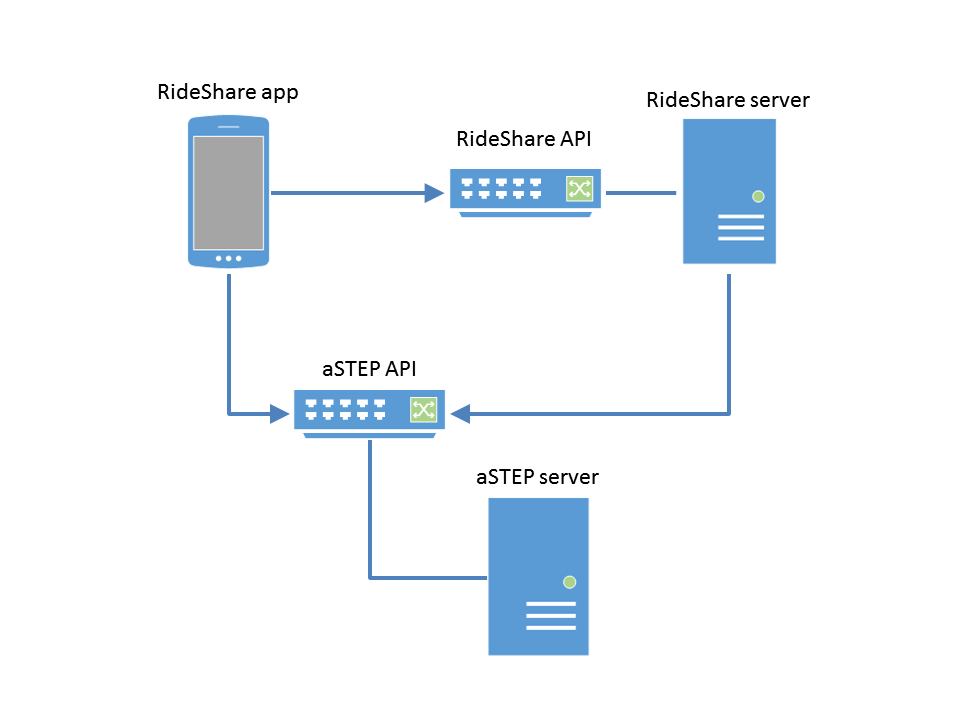
\includegraphics[width=\textwidth]{figures/SystemDesign.png}
	\caption{System design, including all major parts of the solution.}
	\label{fig:s2systemdesign}
\end{figure}


%This means that a user will be represented in the \gls{rs} solution and in the \gls{astep} system. 


% Definition of RIDESHARE(TM) server responsibilities
Beyond storing scores for route matches and additional user info the \gls{rs} server will also be responsibly for sending request to the \gls{astep} server, concerning calculations about stable routes and route matches.
To be able to gain access to each user's location data from \gls{astep}, the \gls{rs} server has to store some sort of login information.
The \gls{astep} system provides a login token, so that a password does not need to be stored on the \gls{rs} server.


% Completed system design
The final system design developed in the second iteration, described in this section, can be seen in Figure \ref{fig:s2systemdesign}.

